
\documentclass[11pt,a4j]{jreport}
\renewcommand{\baselinestretch}{1.4}
\usepackage{comment}
\usepackage{float}
\usepackage{color}
\usepackage{multicol}
%\usepackage[dvipdfmx]{pict2e}
\usepackage{wrapfig}
%\usepackage{graphicx}
\usepackage[dvipdfmx]{graphicx}
\usepackage{bm}
\usepackage{url}
\usepackage{underscore}
\usepackage{colortbl}
\usepackage{tabularx}
\usepackage{fancyhdr}
\usepackage{ulem}
\usepackage{cite}
\usepackage{amsmath,amssymb,amsfonts}
\usepackage{algorithmic}
\usepackage{textcomp}
\usepackage{xcolor}
\usepackage{booktabs}
\usepackage{longtable}
\usepackage[ipaex]{pxchfon}

\usepackage{listings,jvlisting}
\lstset{
  basicstyle={\ttfamily},
  identifierstyle={\small},
  commentstyle={\smallitshape},
  keywordstyle={\small\bfseries},
  ndkeywordstyle={\small},
  stringstyle={\small\ttfamily},
  frame={tb},
  breaklines=true,
  columns=[l]{fullflexible},
  numbers=left,
  xrightmargin=0zw,
  xleftmargin=3zw,
  numberstyle={\scriptsize},
  stepnumber=1,
  numbersep=1zw,
  lineskip=-0.5ex
}
\renewcommand{\lstlistingname}{プログラム}

\usepackage[top=30truemm,bottom=30truemm,left=30truemm,right=30truemm]{geometry}

\begin{document}

\thispagestyle{empty}
\begin{center}
\
\vspace{3cm}

{\huge{Vitis Vision Libraryを用いた前処理の\\
ハードウェア実装と性能評価}}

\vspace{9mm}

{\LARGE 指導教員}

\vspace{5mm}

{\LARGE 高橋 寛 教授}

\vspace{4mm}

{\LARGE 甲斐 博 准教授}

\vspace{4mm}

{\LARGE 王森レイ 講師}

\vspace{20mm}

{\LARGE 令和 5 年 1 月 20 日提出}\\

\vspace{20mm}

{\LARGE 愛媛大学工学部工学科}\\

\vspace{4mm}

{\LARGE 応用情報工学コース}\\

\vspace{4mm}

{\LARGE 計算機/ソフトウェアシステム研究室}\\

\vspace{18mm}

{\huge 西川 竜矢}\\

\end{center}

\thispagestyle{empty}
\clearpage

% 目次の表示
\tableofcontents

%=====================================================================================
\pagestyle{fancy}
\lhead{\rightmark}
\renewcommand{\chaptermark}[1]{\markboth{第\ \normalfont\thechapter\ 章~~#1}{}}
%=====================================================================================
%
%========序論=========================================================================
\chapter{序論} %章

\section{研究背景}

近年,日常生活を送るうえで多くの場面でIoTが活用されている.また,エッジAIの登場により,
IoT機器における処理全体に要する時間の短縮に成功している.その中でも,自動車の歩行者検知や
製造業における外観検査などに使われている技術に物体検出がある.物体検出には高いリアルタイム性
が求められているが,IoT機器におけるエッジデバイスは推論モデルの学習環境に用いられるPCと比較すると
CPU性能やメモリ容量といったリソースが劣る.こうした現状から,限られたリソースの中で,
処理速度やリソース使用量などのパフォーマンスをどれだけ向上させられるかが課題となっている.

また,物体検出に関する研究では,推論処理における高速化が盛んである.その高速化手法\cite{AccelTemp}は,
主流な方法である量子化をはじめ,レイヤフュージョン,デバイス最適化,マルチスレッド化など
さまざまである.しかし,物体検出の流れとしてはじめに入力画像に対する前処理の工程があり,
この工程における高速化の研究は少ない.実際に物体検出の前処理と推論処理では,推論処理に要する
処理時間の方が前処理に要する処理時間より大きくなるのは周知の事実ではあるが,今後さらに
推論処理の高速化が進んでくると,高速化された推論処理に対して,その前に処理速度の遅い前処理の工程が
入ってくるため,折角高速化した推論処理のパフォーマンスを最大限に発揮できなくなってしまう恐れがある.
こうした点から本研究では推論処理の前処理の工程に対して高速化を進めていく.

加えて,エッジコンピューティングにおいて注目すべきはそのエッジデバイスである.
FPGA(Field Programmable Gate Array)は集積回路の一種であり,様々なエッジデバイスに搭載され用いられている.
その大きな特徴として現場で論理回路の構成を書き換え可能である点が挙げられ,こうした特徴から,FPGAはCPUと比較しても
大量のデータを高速に処理し,さらに消費電力が低いという利点がある.以上の点から,リアルタイム性を重要視している
エッジデバイスでの画像処理に対してFPGAを用いることは,先に述べた課題に対する有効的な解決策となるといえる.


\section{論文の構成}
※全体が完成したら書きます.
%本論文ではエッジコンピューティングにおける物体検出の入力画像に対する前処理の高速化について
%本論文の構成について述べる.第1章では研究背景について述べる.第2章では本論文を読むにあたって必要となる予備知識
%について,画像処理およびFPGAの観点から説明する.第3章では本研究で扱う画像処理アプリケーションの実装について,
%開発環境,開発フロー及び
%
%========予備知識=========================================================================
\chapter{予備知識}
本章では,この論文を読むにあたって理解しておく必要のある予備知識について記述する.
\section{画像処理}
\subsection{物体検出}
機械学習を活用して画像に映る特定の物体を検出する技術を物体検出と呼ぶ.
物体検出における大まかな流れを図2.1に示す.
\begin{figure}[H]
  \center
  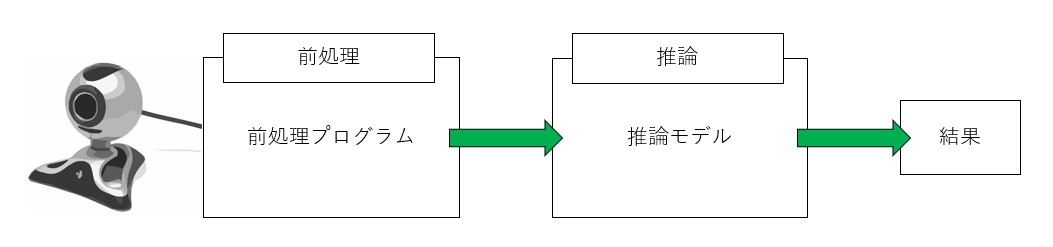
\includegraphics[scale = 0.8]{pict/pict4.jpg}
  \caption{物体検出の流れ}
\end{figure}
物体検出の流れとして,はじめにカメラから入力画像を取得する.
この画像に対して画像前処理を行う.この処理は画像データの整形を行い,整形したデータを
推論モデルに渡す.
整形された画像データを受け取った推論モデルは推論処理を行い,
推論結果を出力する.こうした流れで物体検出技術は実現されており,
製造業や自動車分野,さらには医療分野など幅広い分野で利用されている.

\subsection{物体検出の詳細}
本研究における物体検出の詳細について示す.
本研究では推論モデルに,YOLOv3 tinyおよびYOLOv4を想定しており,
入力画像に対する前処理はリサイズを行う.
\begin{figure}[H]
  \center
  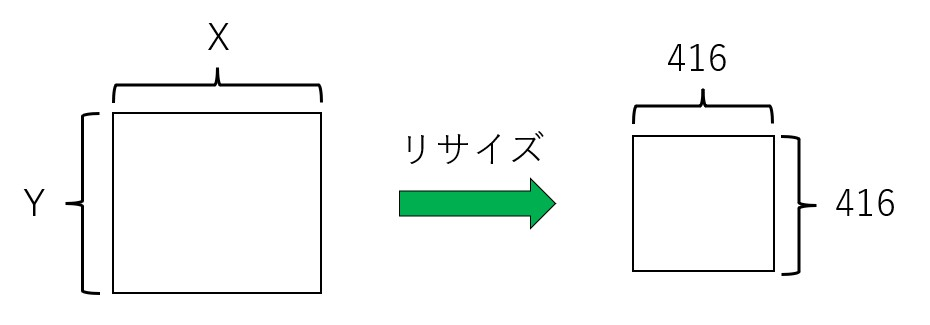
\includegraphics[scale = 0.8]{pict/pict5.jpg}
  \caption{リサイズ}
\end{figure}
図2.2にリサイズの工程を示した.
入力画像のサイズを横:X,縦:Yに対してリサイズ後のサイズは416pxの正方形である.

%次に正規化について示す.正規化とは特徴量の値の範囲を一定の範囲内に収めるように変換する処理のことである.
%\begin{equation}
%  \begin{split}
%  &x_{norm} = \frac{x-x_{min}}{x_{max}-x_{min}} \\
%  (x_{norm}:xを正規化&した値, x_{min}:xの最小値,x_{max}:xの最大値) \\
%  \end{split}
%\end{equation}
%式2.1ではある特徴量xに対して特徴量の取り得る最小値を引き,その値を
%特徴量の最大値と最小値の差つまり特徴量の取り得る範囲で割ることで
%正規化を行っている.これは特徴量の値を0から1の値に変換する処理であることから
%0,1スケーリングと呼ばれる.

\subsection{OpenCV}
OpenCVとはOpen Source Computer Vision Libraryの略称で,Intelが開発した画像・動画に関する処理機能をまとめた
オープンソースのライブラリである.OpenCVの持つ機能\cite{OpenCV}を以下に列挙する.
\begin{quote}
  \begin{itemize}
    \item 画像の入出力
    \item 画像の前処理
    \item 画像内のオブジェクト検出
    \item 画像への描写処理
    \item Deep Learning
  \end{itemize}
\end{quote}

\section{FPGA}
\subsection{FPGA概要}
FPGAはField Programmable Gate Arrayの略称であり,日本語に直訳すると「現場で構成可能なゲートアレイ」となる.
ここで言う「ゲートアレイ」とは,ASIC(Application Specific Integrated Circuit)の設計・製造手法のひとつである.
この手法では,ウェハ―上に標準NANDゲートやNORゲート等の論理回路,単体のトランジスタ,抵抗器などの受動素子といった部品を
決まった形で配置し,その上に配線を加えることで各部品を配線し半導体回路を完成させる.昨今では専用LSIであるASICの開発に
数千万円から数億円の初期コストがかかることや,一度製造してしまったLSIの構成は製造後には変更できないなどの問題がある.
一方でFPGAは「現場で構成可能」という表現からもわかる通り,ユーザの手元でロジックや配線を変更できるというコンセプトを基に
開発される.現在開発されているFPGAの規模は様々だが,一昔前の専用LSIを超える規模の回路を簡単に構成できるようになってきている.
また,FPGAとASICなどの専用LSIとの大きな違いとして「製造のための初期コスト」が不要なことも挙げられる.
\subsection{Ultra96v2}
本研究で扱うFPGAボード.Ultra96v2に搭載されているZynq UltraScale+ MPSoC\cite{boardinfo}は,プロセッサとFPGAを
1チップに搭載しており,機能を以下に述べる.
%引用https://www.avnet.com/wps/portal/japan/products/product-highlights/ultra96/
\begin{quote}
  \begin{itemize}
    \item 高性能かつ大容量プログラムロジックを利用した高帯域な信号・画像処理
    \item Cortex-A53アプリケーションプロセッサで余裕のあるシステム(OS/GUI)プロセス処理実行
    \item Cortex-R5でタイミングクリティカルなリアルタイム処理をプログラムロジックと連携処理
  \end{itemize}
\end{quote}
以上の機能を持つことからも,自動車,医療,製造業,放送,通信などの幅広い分野で利用されている.

\section{ハードウェアアクセラレーション}
通常,CPU(PS:Processing System)によって処理されるプログラムが,処理速度や消費電力など課題を抱えている場合に,
こうした処理のための専用ハードウェア(PL:Programmable Logic)を構成することで処理を援助し,高速化を図る手法のこと.

本研究では,物体検出における前処理に対してハードウェアアクセラレーションをすることで,処理の高速化を図る.
%
%========エッジAIプラットフォーム開発=================================================================
\chapter{エッジAIプラットフォーム開発}
\section{Vitis プラットフォーム概要}
Vitis プラットフォームは,外部メモリインターフェイス,カスタム入出力インターフェイス,ソフトウェアランタイムなど,
AMDザイリンクスプラットフォームのハードウェアやソフトウェアのベースアーキテクチャおよびアプリケーションコンテキストを
定義する.

Vitis プラットフォーム\cite{VitisPlatform}を使用する設計書法は様々なメリットをもたらし,生産性の向上につながる.特徴を以下に列挙する.
\begin{quote}
  \begin{itemize}
    \item プラットフォームの再利用性:同じプラットフォーム上で異なるアクセラレーションアプリケーションを入れ替え可能
    \item アプリケーションの移植性:最小限の操作で異なるプラットフォーム間でアプリケーションを移植可能
    \item シミュレーション時間:カーネルを使用する協調シミュレーションの高速化
    \item ランタイム:オープンソースのランタイムを使用してPCle®インターフェイスまたはエンベデッドインターフェイス経由でホストとデバイス間の通信を制御
    \item システムデバッグ:システム全体の協調シミュレーションによって,全ハードウェアコンパイル時間を短縮
  \end{itemize}
\end{quote}
\section{Vitis プラットフォーム開発環境とツール}
\begin{quote}
  \begin{itemize}
    \item Ubuntu18.04.3 LTS・・・
    LinuxOSのUbuntuを用いた.開発ツールであるVivado,PetaLinux,Vitisのバージョンに対応させてUbuntuのバージョンは
    18.04を採用している.
    \item Vivado-v2020.1・・・
    Xilinxが提供するハードウェア設計ツール.HDLからビットストリームの生成,FPGAへの書き込みまでの開発における下位の部分
    を担当する.
    \item PetaLinux-v2020.1・・・
    Xilinxが提供するツール.Xilinxのプロセッシングシステム上で組み込みLinuxのソリューションをカスタマイズ,ビルド,
    およびデプロイするために必要なモノを全て提供する.設計生産性の加速を目的とするこのソリューションは,Xilinxの
    ハードウェア設計ツールと連動し,Versal,Zynq UltraScale+ MPSoP,Zynq-7000,およびMicroBlaze向けのLinuxシステム
    の開発を容易にする.
    \item Vitis-v2020.1・・・
    Xilinxが提供するVitis統合ソフトウェアプラットフォーム.ツール内容を以下に述べる.
    \begin{quote}
      \begin{itemize}
        \item アクセラレーションアプリケーションをシームレスに構築するための包括的なコア開発キット
        \item AMDザイリンクスのFPGAおよびVersa I ACAPハードウェアプラットフォーム向けに最適化された,
        ハードウェアアクセラレーション用の豊富なオープンソースライブラリ
        \item 使い慣れた高レベルのフレームワークを利用して直接開発できる,プラグインタイプのドメイン特化開発環境
        \item 今後さらに拡大する,ハードウェアアクセラレーションパートナー提供のライブラリおよび構築済みアプリケーション
        のエコシステム
      \end{itemize}
    \end{quote}
    %\item OpenCV-v3.4.16・・・
    %本研究で扱うVitis-v2020.1が用いるVitis Vision Libraryに対応しているバージョンのOpenCVを用いる.
  \end{itemize}
\end{quote}
\section{Vitis プラットフォーム作成}
\begin{figure}[H]
  \center
  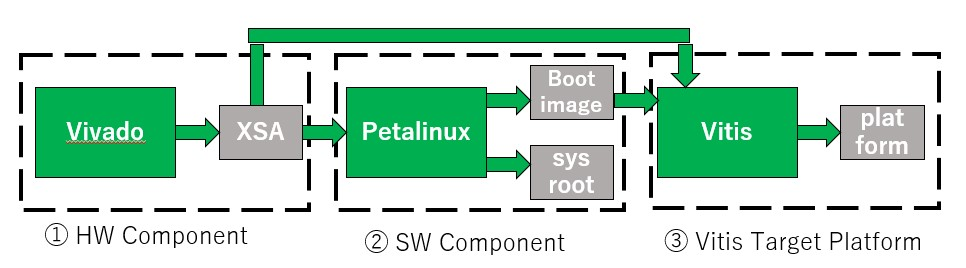
\includegraphics[scale = 0.8]{pict/pict.jpg}
  \caption{プラットフォーム作成フロー}
\end{figure}
プラットフォームの作成は図3.1プラットフォーム作成フローに従って行い,
以下に示す工程はXilinx提供のユーザガイド\cite{Xilinx-platform}を参考にして実行する.
また,Ultra96v2向けプラットフォームがavnet社より提供されているので,
このプラットフォームを用いても良いのだが,カーネル作成時にライブラリの
追加などを行う必要があるため,avnet社が提供しているプラットフォームの内,
ハードウェア構成が構築されているXSAファイルのみを引用する.そのため,
1.HW Componentの工程は省略する.図3.2に引用するXSAファイルのBlockDesignを示す.
\begin{figure}[H]
  \center
  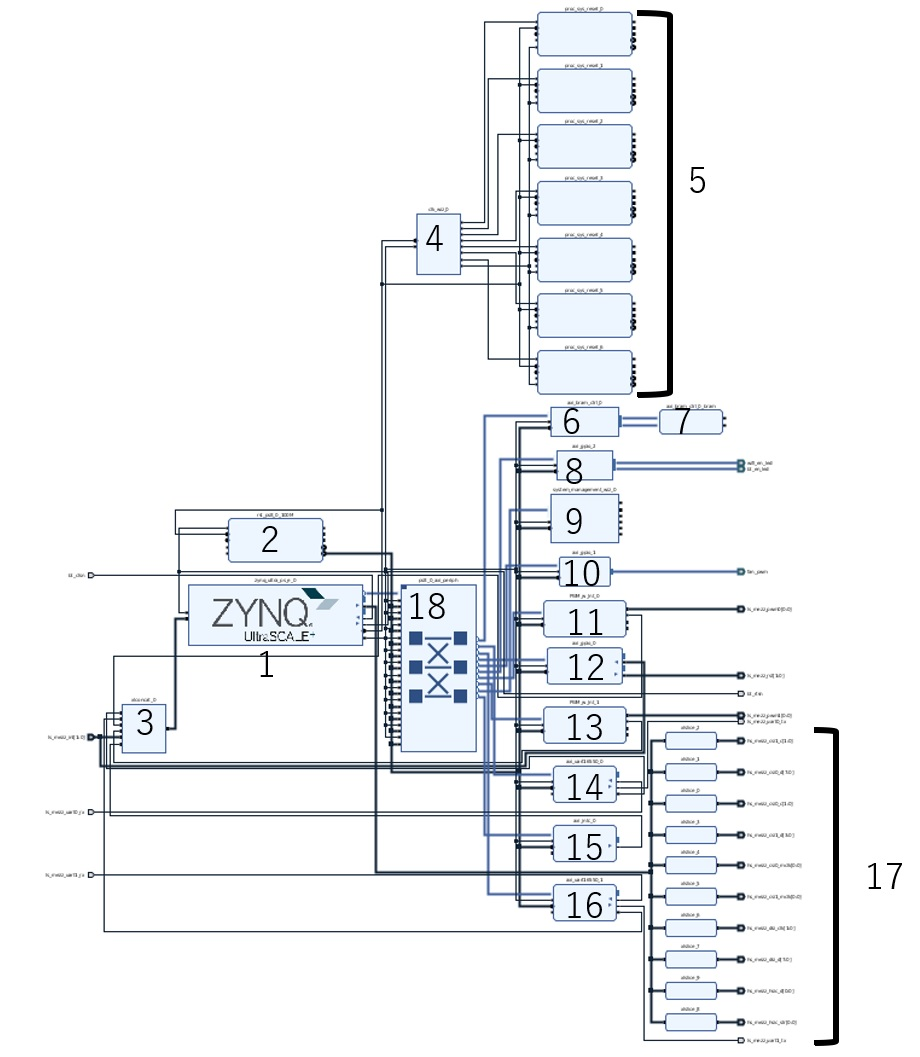
\includegraphics[scale = 0.8]{pict/pict2.jpg}
  \caption{HW BlockDesign}
\end{figure}
図3.2中の配線によって繋がれているブロックの部分をIP(Intellectual Property)
と呼び,FPGA業界では,既に設計された設計資産,の意味で使用される.
回路設計を行うユーザの視点からすると,既に設計された回路ライブラリを表す.
こうしたIPを利用することにより,容易な回路設計を実現している.
図3.2に示したBlockDesignの各IPを表3.1に列挙する.
\begin{table}[H]
  {\scriptsize
  \caption{BlockDesignにおけるIP}
  \label{table:SpeedOfLight}
  \centering
   \begin{tabular}{clll}
    \hline
    番号 & IP種類 & IP名称 & 出力端子 \\
    \hline \hline
    1 & Zynq UltraScale++ MPSoC & zynq_ultra_ps_e_0 & \\
    2 & Processor System Reset & rst_ps8_0_100M & \\
    3 & Concat & xlconcat_0 & \\
    4 & Clocking Wizard & clk_wiz_0 &\\
    5 & Processor System Reset & proc_sys_reset_0 & \\
     & Processor System Reset & proc_sys_reset_1 & \\
     & Processor System Reset & proc_sys_reset_2 & \\
     & Processor System Reset & proc_sys_reset_3 & \\
     & Processor System Reset & proc_sys_reset_4 & \\
     & Processor System Reset & proc_sys_reset_5 & \\
     & Processor System Reset & proc_sys_reset_6 & \\
    6 & AXI BRAM Controller & axi_bram_ctrl_0 & \\
    7 & Block Memory Generator & axi_bram_ctrl_0_bram & \\
    8 & AXI GPIO & axi_gpio_2 & wifi_en_led, bt_en_led\\
    9 & System Management Wizard & system_management_wiz_0 & \\
    10 & AXI GPIO & axi_gpio_1 & fan_pwm \\
    11 & & PWM_w_lnt_0 & ls_mezz_pwm0[0:0] \\
    12 & AXI GPIO & axi_gpio_0 & ls_mezz_rst[1:0] \\
    13 & & PWM_w_lnt_1 & ls_mezz_pwm1[0:0] \\
    14 & AXI UART166550 & axi_uart166550_0 & ls_mezz_uart0_tx \\
    15 & AXI Interrupt Controller & axi_intc_0 & \\
    16 & AXI UART166550 & axi_uart166550_1 & ls_mezz_uart0_tx \\
    17 & Slice & xlslice_0 & hs_mezz_csi0_c[1:0] \\
    & Slice & xlslice_1 & hs_mezz_csi0_d[7:0] \\
    & Slice & xlslice_2 & hs_mezz_csi1_c[1:0] \\
    & Slice & xlslice_3 & hs_mezz_csi1_d[3:0] \\
    & Slice & xlslice_4 & hs_mezz_csi0_c[1:0] \\
    & Slice & xlslice_5 & hs_mezz_csi1_d[3:0] \\
    & Slice & xlslice_6 & hs_mezz_dsi_mclk[0:0] \\
    & Slice & xlslice_7 & hs_mezz_dsi_clk[1:0] \\
    & Slice & xlslice_8 & hs_mezz_dsi_d[7:0] \\
    & Slice & xlslice_9 & hs_mezz_hsic_d[0:0] \\
  \hline
  \end{tabular}
  }
\end{table}
FPGAではFPGA内部のロジックに供給するクロックを指定する必要がある.
その機能を有しているIPが図3.2中の4番目のIPであるClocking Wizardであり,
実際に出力されるクロックの詳細について表3.2に示す.
\begin{table}[H]
  \caption{Clocking Wizardによる出力クロック}
  \label{physics}
  \centering
  \begin{tabular}{ccc}
    \hline
    ポート名 & \multicolumn{2}{c}{出力周波数 (MHz)} \\
    \cmidrule(lr){2-3}
     & 要求 & 実際 \\
    \hline
    clock_out1 & 150 & 150 \\
    clock_out2 & 300 & 300 \\
    clock_out3 & 75 & 75 \\
    clock_out4 & 100 & 100 \\
    clock_out5 & 200 & 200 \\
    clock_out6 & 400 & 400 \\
    clock_out7 & 600 & 600 \\
    \hline
    \end{tabular}
\end{table}

2.SW Componentの工程に移る.この工程ではPetalinuxツールを用いて作業を行う.
はじめに,petalinux projectを作成する.ここでは,後のカーネルおよびrootfsの設定を省略するため
avnet社の提供しているUltra96v2専用のBoard Support Packageファイルを用いてプロジェクトを立ち上げる.
次に1.HW Componentで示したXSAファイルからハードウェアコンポーネントの情報を取り込む.
最後にrootfsの設定として,利用するuser package,opencv,pythonのライブラリを有効にする.
以上の設定を経て,PetaLinuxプロジェクトのビルドを行う.ビルドを行うことで,設定したLinuxカーネル並びにsdk.shの生成を行う.
生成したsdk.shを自己解凍することでsysrootが生成される.
以下に2.SW Componentにおける成果物のうち,後のVitis Target Platformの作成とVitis applicationの作成で
用いるファイルおよびディレクトリを列挙する.
\begin{quote}
  \begin{itemize}
    \item bl31.elf
    \item image.ub
    \item pmufw.elf
    \item u-boot.elf
    \item fsbl.elf
    \item system.dtb
    \item linux.bif
    \item rootfs.ex4
    \item sysroot
  \end{itemize}
\end{quote}
上記の生成物の内,bl31.elf,image.ub,pmufw.elf,u-boot.elf,fsbl.elf,system.dtb,linux.bifを
bootディレクトリにまとめて管理する.

1.HW Componentと2.SW Componentの工程で得られた成果物とVitisツールを用いて
Vitis Target Platformの作成を行う.Vitisを起動後,1.HW Componentで示したXSAファイルを選択して,
Platform Projectを作成する.Domein設定を開き,OSをLinux,Processorをpsu_cortex53に指定する.
加えてBifファイルをlinux.bif,Boot Components DirectoryおよびLinux Image Directoryをbootディレクトリ,
rootfs fileをrootfs.ex4,Sysroot Directoryにsysroots/aarch64-xilinx-linuxディレクトリを指定した.
最後にBoard Support Packageの設定を行い,プラットフォームをビルドすることでプラットフォーム作成を完了する.

\section{Vitis Vision Library}
FPGA用の画像データ前処理アプリケーションはVitisというツールで作成するため,Vitisツール専用のライブラリを用いる必要がある.
そのライブラリが,Xilinxから提供されているVitis Vision Libraryであり,OpenCVの画像処理関数の多くを含んでいる.
Vitis Vision Libraryの特徴を以下に列挙する.
\begin{quote}
  \begin{itemize}
    \item 色およびビット深度変換,ピクセルごとの算術演算,幾何変換,統計,フィルター,特徴検出,分類,3D再構成など性能に最適化された機能の提供
    \item カラー画像処理のネイティブサポート,マルチチャネルストリーミングのサポート
    \item オンチップメモリまたは外部メモリ間のデータ移動を効率的に管理して最大限の性能を達成
    \item ビジョンパイプラインに求められる演算能力をすばやく評価して最適なデバイスを選択
    \item ビジョンおよび画像処理アルゴリズムを高速化する方法を示すサンプルデザインを提供
    \item 関数パラメータを活用し,1クロックサイクルで複数ピクセルを処理してスループット要件を満たす
  \end{itemize}
\end{quote}
%
%========アプリケーションの実装=================================================================
\chapter{アプリケーションの実装}
本研究では物体検出における画像前処理アプリケーションを作成する.
PSのみを利用して処理を行うアプリケーションと
PSとPLを用いて処理を行うアプリケーションの作成を行う.
\section{アプリケーション作成(PS)}
実行時にPSのみを用いて画像の前処理を行うアプリケーションの作成について述べる.
このアプリケーションのソースコードはPythonで記述しており,
ファイル名をprepro_PS.pyとし以下に示す.
\begin{lstlisting}[caption=prepro_PS.py]
  import glob
  import sys
  import time
  import cv2
  import numpy as np
  
  re_length = 416
  total = 0
  
  for i in range(600):
  
      img = cv2.imread("./mask_before/Mask_" + str(i+1) + ".jpg")
  
      time_sta = time.time()
  
      h, w = img.shape[:2]
  
      re_h = re_w = re_length/max(h,w)
  
      img_resize = cv2.resize(img, dsize=None, fx=re_h, fy=re_w)
  
      time_end = time.time()
      t = time_end - time_sta
      total = total + t
  
  print("time:" + str(total) + "[ms]")
\end{lstlisting}
prepro_PS.pyの概要を以下に述べる.
1行目から5行目までは必要なモジュールを利用するための記述である.
7行目の変数re_lengthは入力画像に対してリサイズした後の画像サイズ
である416pxを定義している.ここでは入力画像の長辺を416pxにリサイズ
することを想定しており,リサイズ後も長辺と短辺の大きさの比率は変わらない.
10行目から20行目までの画像処理の部分の説明をする.
前処理を行うサンプル画像の枚数は600枚で行ったので10行目のrangeの中は
600に指定している.12行目ではopencvを利用した入力画像の取得を行っており,
続けて16行目で入力画像の縦のサイズ:h,横のサイズ:wを取得している.
18行目では入力画像を変換する倍率の計算を行っており,リサイズ後の長辺サイズである
416pxを入力画像の縦,横のピクセルサイズのうち大きい方で除算することにより倍率を計算している.
20行目のimg_resizeには入力画像をリサイズした後の配列を格納する.
opencvの関数であるcv2.resizeに対して入力画像imgと18行目で計算した倍率である
re_hとre_wを引数として渡すことでリサイズ処理を行う.

リサイズにかかる処理時間は,変数totalに格納する.リサイズの処理を行う前後で
時刻を取得し,その処理時間の計算を行う.1枚当たりにかかった処理時間を変数totalに
加算していくことで,最終的に600枚当たりの処理時間の計測を行っている.
%21行目のimg_normalは正規化後の画像配列を格納する.正規化とは,
%複数あるデータのうち,そのデータの取り得る最大値と最小値の差で
%各データを除算する.今回は,画像配列に対して正規化を行うため,
%その配列の要素の取り得る範囲は0から255である.そのため,21行目では
%リサイズ後の画像配列であるimg_resizeを255で除算することにより正規化を
%行っている.

\section{アプリケーション作成(PS+PL)}
PSとPLを用いるアプリケーションの作成は,3章で作成したプラットフォームを利用して行う.
Vitisを起動し,プラットフォームの選択を行い,その後サンプルからVitis Vision Libraryの
resizeを選択する.作成したソースコードを以下に示す.

※完成したら書きます

%
%========ここにC++で記述されたリサイズのソースコードを貼る.
%
%========ここにソースコードの説明
%
アプリケーションの作成が完了すると新たにSD_Card.imgが生成される.
%========評価実験=======================================================================
\chapter{評価実験}
\section{実験準備}
\subsection{データセット}
実験に用いるサンプル画像は,Vitis-AIのUltra96v2上動作に関する記事\cite{SamplePictWeb}に記載されている
マスクを着用している人々の画像データセットであるMask Dataset\cite{SamplePictDrive}を利用した.
このデータセットの内,600枚の画像に対して前処理プログラムを実行する.サンプル画像の例を図5.1に示す.
\begin{figure}[H]
  \center
  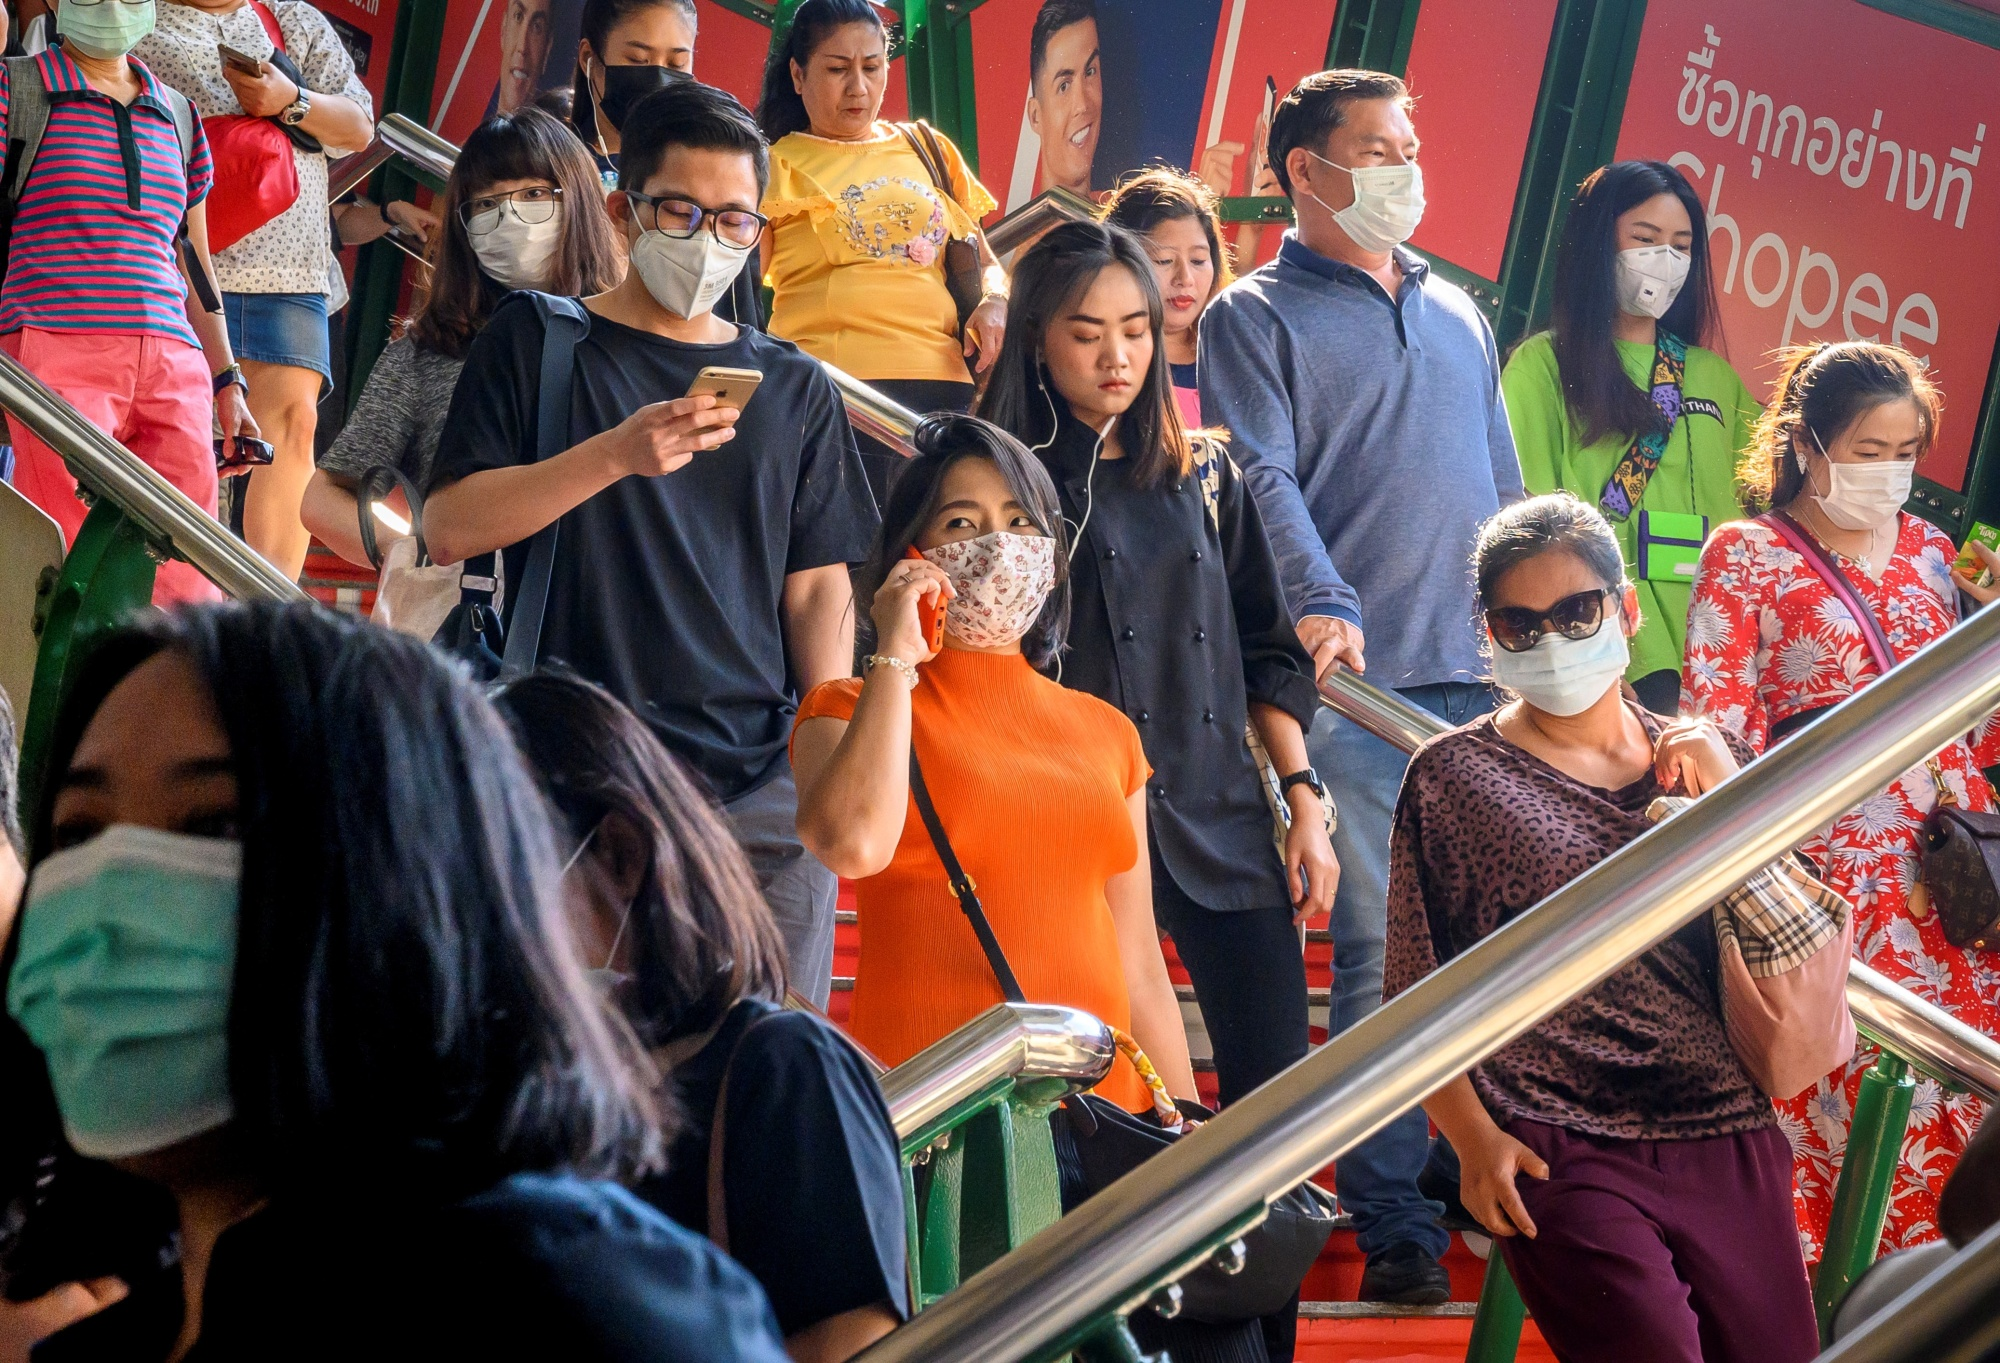
\includegraphics[scale = 0.17]{pict/Mask_1.jpg}
  \caption{Mask Dataset Sample Picture}
\end{figure}

\subsection{SD_Cardの作成}
Ultra96v2で扱うMicroSDカードに,作成したデータを書き込む方法について図5.2に示す.
\begin{figure}[H]
  \center
  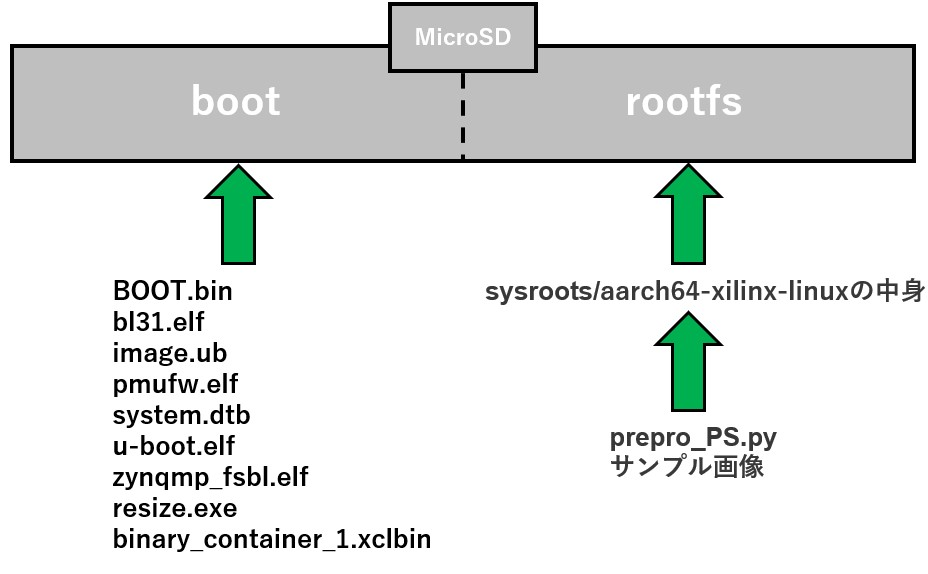
\includegraphics[scale = 0.7]{pict/pict6.jpg}
  \caption{Mask Dataset Sample Picture}
\end{figure}
作成したデータの書き込みにはbalenaEtcherというツールを用いる.このツールを用いてSD_Card.imgをMicroSDカードに書き込むことで
自動的にMicroSDカードのパーミッションが割り当てられる.
MicroSDカードに書き込まれたデータを以下に列挙する.
※実際に書き込んだら記述します.
%ディレクトリパスを記述します
%4章で作成したSD_Cardディレクトリの中身をMicroSDカードの第1パーティション(ディレクトリ名:boot)に,
%3章のSW Componentで作成したsysrootディレクトリの中のaarch64-xilinx-linuxディレクトリの中身をMicroSDカードの
%第2パーティション(ディレクトリ名:rootfs)に書き込む.ここで,PSとPLを用いて処理を行うアプリケーションは,
%/ディレクトリパス/の中に,PSのみを用いて処理を行うアプリケーションはhomeディレクトリの中に書き込む.
%加えて前処理を行うサンプル画像について記述する.

\subsection{実験環境の構築}
必要なファイルの書き込みが完了したので,MicroSDカードをUltra96v2に挿入し,PCとシリアル通信を行う.
シリアル通信用ツールであるGTKtermを起動し,設定画面を開き,ポートを/dev/ttyUSB1に,ボーレートを115200に指定した.
Ultra96v2の起動ボタンを押すと,Linuxカーネルが起動する.
加えて,はじめにPSのみを用いて処理を行うアプリケーションのために,pythonで用のOpenCVをダウンロードする.
\section{アプリケーションの実行}
※実行したら書きます.
\section{実験結果}
※結果出たら書きます.
%
%========考察========================================================================
\chapter{考察}
本章では,ハードウェア実装した前処理の性能に対する考察と,本研究の今後の展望についての考察を述べる.

まず,ハードウェア実装した前処理の性能に対する考察を述べる.
※実験終わったら書きます

次に,本研究の今後の展望について考察を述べる.本研究では,物体検出における前処理の部分の中でも,
特にリサイズの処理に対して焦点を当てた.しかし実際の前処理では,リサイズだけの処理をするわけではなく,
正規化などの他の処理も行う,この前処理は推論モデルによってまちまちである.そのため,リサイズ以外の前処理についても
ハードウェア実装をすることで高速化できると考える.
また,エッジコンピューティングにおける速度以外の課題であるリソースの使用率や消費電力の項目についてもハードウェア化することで
どのような変化をもたらすか検証する必要がある.
加えて,ハードウェア実装した前処理を,物体検出に組み込み,前処理から推論処理までの物体検出全体の処理速度にどの程度影響を
及ぼすのかも検証する必要がある.
%=======あとがき=====================================================================
\chapter{あとがき}
本研究では,物体検出におけるリアルタイム性を課題として取り上げ,前処理を高速化することを目的とした.
この目的を成し遂げるため,前処理の部分をハードウェア実装することを目標とした.
本研究を進めるにあたって,はじめに開発ツールであるVivado,Petalinux,Vitisの使用方法について学習を行った.
その後,プラットフォームの作成,アプリケーションの作成,FPGAボードでの実験,性能評価の順で実行した.

本研究の結果
※実験終わったら書きます

しかし,ハードウェア実装できた前処理はリサイズ処理のみであり,さらに高速化を図るためには,その他の前処理についても
ハードウェア実装する必要がある.加えてエッジデバイスにおけるリアルタイム性以外の課題であるリソース使用率や消費電力については
検証できていないのため,これらの項目についても検証する必要がある.
%また,先に述べた開発ツールを利用するにあたって,ハードウェアとソフトウェアの開発に関する知識の両方が必要となるため,
%ツールを扱えるようになるまで多くの時間を必要とする.
以上を今後の課題とし,解決することでエッジデバイスにおける物体検出のリアルタイム性向上につながると考える.

%=====================================================================================
\chapter*{謝辞} %章を付けずにタイトル表示
\addcontentsline{toc}{chapter}{謝辞} %章立てせずに目次に追加するおまじない
本研究,論文作成を進めるにあたり,御懇篤な御指導,御鞭撻を賜りました本学高橋寛教授ならびに
甲斐博准教授,王森レイ講師に深く御礼申し上げます.

また,審査頂いた本学()教授ならびに()助教授に深く御礼申し上げます.

最後に,多大な御協力と貴重な御助言を頂いた計算機/ソフトウェアシステム研究室の諸氏に厚く御礼申し上げます.
%=====================================================================================
%\chapter*{参考文献}
\addcontentsline{toc}{chapter}{参考文献} %章立てせずに目次に追加するおまじない
\renewcommand{\bibname}{参考文献} %これがないと,タイトルが「関連図書」になってしまう
\bibliography{bibtexファイル名} %bibtexファイルの読み込み
\bibliographystyle{junsrt} %本文に\cite{}を入れることで,参考文献表示
\begin{thebibliography}{99}
  \bibitem{AccelTemp} 小西祥之,国宗大介,西田芳隆,ミラクシアエッジテクノロジー株式会社, \\2021, \\"物体検出におけるエッジ環境での推論高速化と精度上昇", \\\url{https://www.jstage.jst.go.jp/article/pjsai/JSAI2021/0/JSAI2021_3I4GS7a02/_pdf/-char/ja}, \\(参照2023-01-19)
  \bibitem{OpenCV} ケイエイブル株式会社, \\"初めてのOpen CV(画像処理ライブラリ)ガイド" \\\url{https://www.klv.co.jp/corner/python-opencv-what-is-opencv.html}, \\(参照2023-01-19)
  \bibitem{boardinfo} AVNET, \\"Ultra96開発ボードでXilinx Zynq UltraScale+ MPSoCを手軽に評価", \\\url{https://www.avnet.com/wps/portal/japan/products/product-highlights/ultra96/}, \\(参照2023-01-19)
  \bibitem{VitisPlatform} Xilinx, \\"Vitis 統合ソフトウェアプラットフォーム,プラットフォームベースフロー", \\\url{https://japan.xilinx.com/products/design-tools/vitis/vitis-platform.html}, \\(参照2023-01-19)
  \bibitem{Xilinx-platform} Xilinx, \\"Vitis 統合ソフトウェアプラットフォームの資料:エンベデッドソフトウェア開発", \\2020-06-24, \\\url{https://docs.xilinx.com/r/2020.1-日本語/ug1400-vitis-embedded}, \\(参照2023-01-18)
  \bibitem{SamplePictWeb} Qiita, \\"Vitis-AI v1.4 on Ultra96v2", \\2021-11-06, \\url{https://qiita.com/lp6m/items/4117a3bab185afedfd5f}, \\(参照2023-01-19)
  \bibitem{SamplePictDrive} Google Drive, \\"Mask_Dataset", \\2020-02-26, \\url{https://drive.google.com/drive/folders/1aAXDTl5kMPKAHE08WKGP2PifIdc21-ZG}, \\(参照2023-01-19)
\end{thebibliography}
\end{document}